\HeadingLevelB{The IBM 4765 Secure Coprocessor}

Secure coprocessors~\cite{yee1994coprocessors} encapsulate an entire computer
system, including a CPU, a cryptographic accelerator, caches, DRAM, and an I/O
controller within a tamper-resistant environment. The enclosure includes
hardware that deters attacks, such as a Faraday cage, as well as an array of
sensors that can detect tampering attempts. The secure coprocessor destroys the
secrets that it stores when an attack is detected. This approach has good
security properties against physical attacks, but tamper-resistant enclosures
are very expensive~\cite{anderson2001security}, relatively to the cost of a
computer system.

The IBM 4758~\cite{smith1999ibm4758}, and its most current-day successor, the
IBM 4765~\cite{nist2015ibm4765} (shown in Figure~\ref{fig:ibm_4765}) are
representative examples of secure coprocessors. The 4758 was certified to
withstand physical attacks to FIPS 140-1 Level 4~\cite{smith1999validating},
and the 4765 meets the rigors of FIPS 140-2 Level 4~\cite{nist2011fipscert}.

\begin{figure}[hbt]
  \centering
  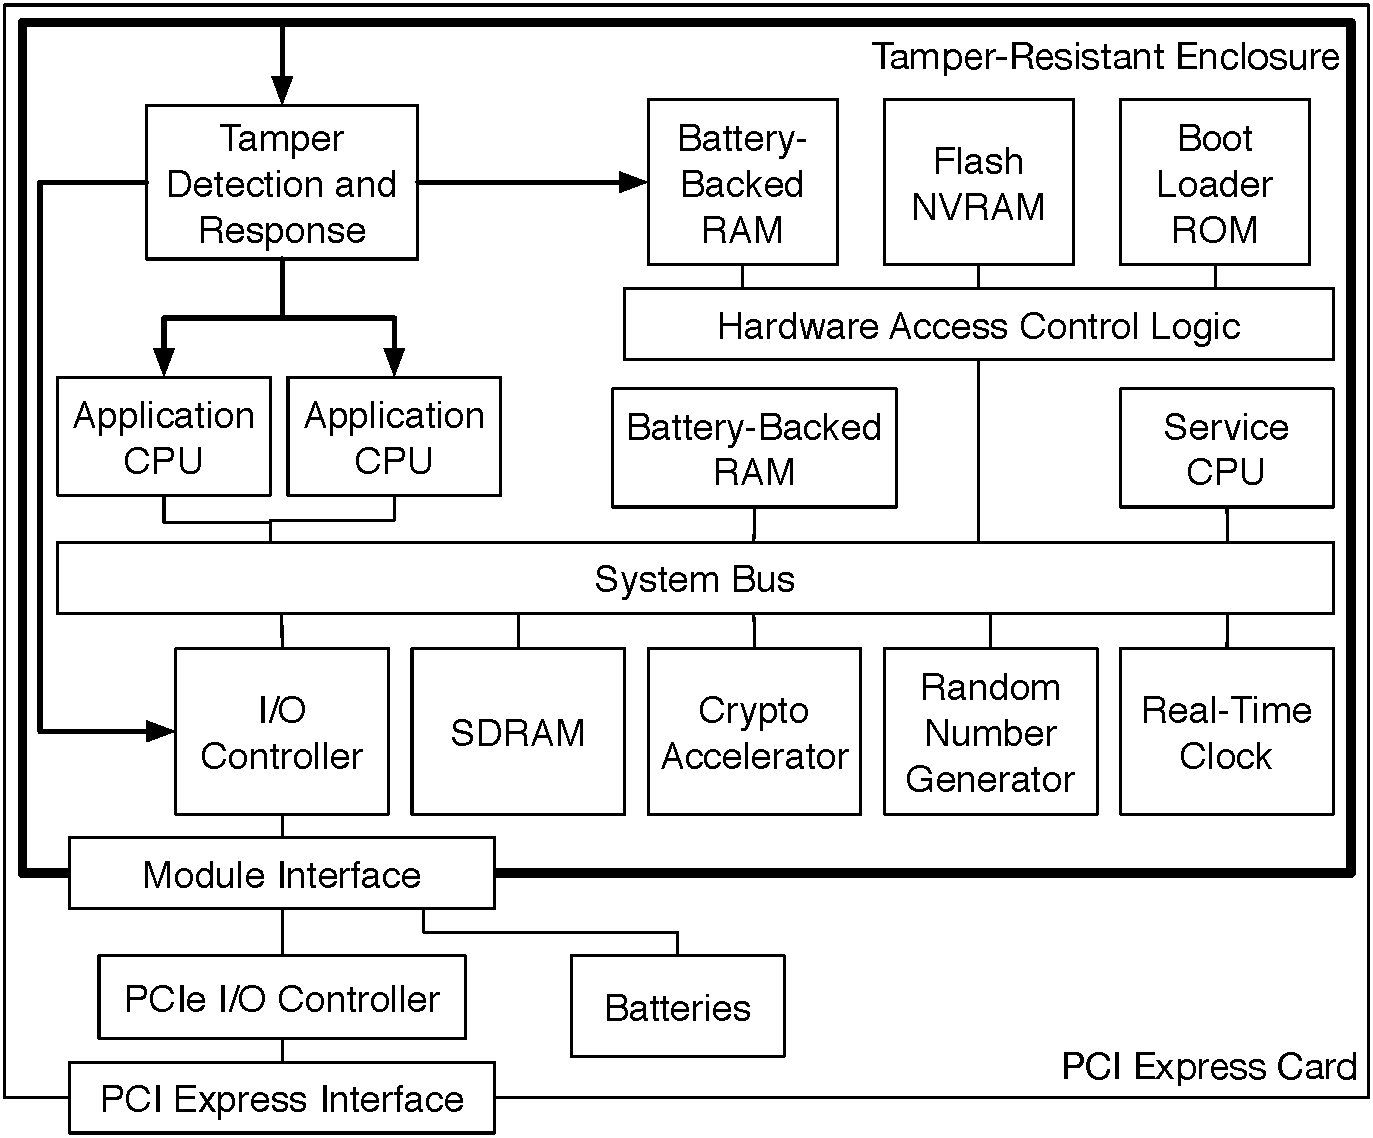
\includegraphics[width=85mm]{figures/ibm_4765.pdf}
  \caption{
    The IBM 4765 secure coprocessor consists of an entire computer system
    placed inside an enclosure that can deter and detect physical attacks.
    The application and the system use separate processors. Sensitive memory
    can only be accessed by the system code, thanks to access control checks
    implemented in the system bus' hardware. Dedicated hardware is used to clear
    the platform's secrets and shut down the system when a physical attack is
    detected.
  }
  \label{fig:ibm_4765}
\end{figure}

The 4765 relies heavily on physical isolation for its security properties. Its
system software is protected from attacks by the application software by
virtue of using a dedicated service processor that is completely separate from
the application processor. Special-purpose bus logic prevents the application
processor from accessing privileged resources, such as the battery-backed
memory that stores the system software's secrets.

The 4765 implements software attestation. The coprocessor's attestation key is
stored in battery-backed memory that is only accessible by the service
processor. Upon reset, the service processor executes a first-stage bootloader
stored in ROM, which measures and loads the system software. In turn, the
system software measures the application code stored in NVRAM and loads it into
the DRAM chip accessible to the application processor. The system software
provides attestation services to the application loaded inside the coprocessor.
